\documentclass[aspectratio=169]{beamer}

% =========================
% THEME & PACKAGES
% =========================
\usetheme{Madrid}
\usecolortheme{default}
\usefonttheme{professionalfonts}

\usepackage{graphicx}
\usepackage{booktabs}
\usepackage{amsmath}

% =========================
% TITLE INFO
% =========================
\title[FINS Integration in FUXA]%
{Integration of the FINS Protocol into the Open-Source HMI System FUXA}

\author[D. Chrisnanda et al.]%
{Denny Chrisnanda \and Frans Sebastian \and Gilang Hansagita}

\institute[Binus University]%
{Bina Nusantara University}

\date{IEEE Conference Presentation}

% =========================
\begin{document}

% =========================
% TITLE SLIDE
% =========================
\begin{frame}
  \titlepage
\end{frame}

% =========================
% OUTLINE
% =========================
\begin{frame}{Outline}
\begin{itemize}
  \item Motivation and Problem Statement
  \item Research Questions and Contributions
  \item Related Works
  \item System Architecture and Methodology
  \item Implementation and Experimental Setup
  \item Results and Discussion
  \item Conclusions and Future Work
\end{itemize}
\end{frame}

% =========================
% MOTIVATION
% =========================
\begin{frame}{Motivation}
\begin{itemize}
  \item Omron PLCs dominate production lines at PT~XYZ ($>90\%$ machines).
  \item Factory Interface Network Service (FINS) is the de facto Omron protocol.
  \item Commercial HMI/SCADA systems are costly and vendor-locked.
  \item Open-source HMI FUXA lacks native FINS support.
\end{itemize}
\end{frame}

% =========================
% PROBLEM STATEMENT
% =========================
\begin{frame}{Problem Statement}
\begin{itemize}
  \item Lack of native FINS support prevents FUXA adoption in Omron-centric plants.
  \item Middleware-based solutions increase latency and complexity.
  \item Alarm and real-time visualization reliability are critical requirements.
\end{itemize}
\end{frame}

% =========================
% RESEARCH QUESTIONS
% =========================
\begin{frame}{Research Questions}
\begin{block}{RQ1}
How can FINS protocol support be implemented in FUXA with reliability and feature parity comparable to built-in protocols?
\end{block}

\begin{block}{RQ2}
How can stable, low-latency read/write operations be achieved for real-time visualization?
\end{block}
\end{frame}

% =========================
% CONTRIBUTIONS
% =========================
\begin{frame}{Main Contributions}
\begin{itemize}
  \item First native integration of Omron FINS into the FUXA HMI platform.
  \item Backend driver (\texttt{DeviceFins}) and frontend configuration support.
  \item Empirical evaluation of latency, reliability, resource usage, and alarms.
  \item Identification of alarm latency bottleneck in polling-based HMI systems.
\end{itemize}
\end{frame}

% =========================
% RELATED WORKS
% =========================
\begin{frame}{Related Works}
\begin{itemize}
  \item Open-source SCADA using Node-RED, Grafana, InfluxDB.
  \item Web-based HMI platforms (FUXA, OpenPLC testbeds).
  \item Protocol integration studies: Modbus, OPC UA, DNP3.
\end{itemize}
\end{frame}

% =========================
% RESEARCH GAP
% =========================
\begin{frame}{Research Gap}
\begin{itemize}
  \item Existing studies focus on Modbus, OPC UA, MQTT.
  \item No native open-source HMI support for Omron FINS found.
  \item Alarm latency and polling effects rarely analyzed explicitly.
\end{itemize}
\end{frame}

% =========================
% METHODOLOGY OVERVIEW
% =========================
\begin{frame}{Methodology Overview}
\begin{itemize}
  \item Iterative development approach:
  \begin{itemize}
    \item Requirements analysis
    \item System design
    \item Implementation
    \item Experimental evaluation
  \end{itemize}
\end{itemize}
\end{frame}

% =========================
% RESEARCH FLOW
% =========================
\begin{frame}{Research Workflow}
\centering
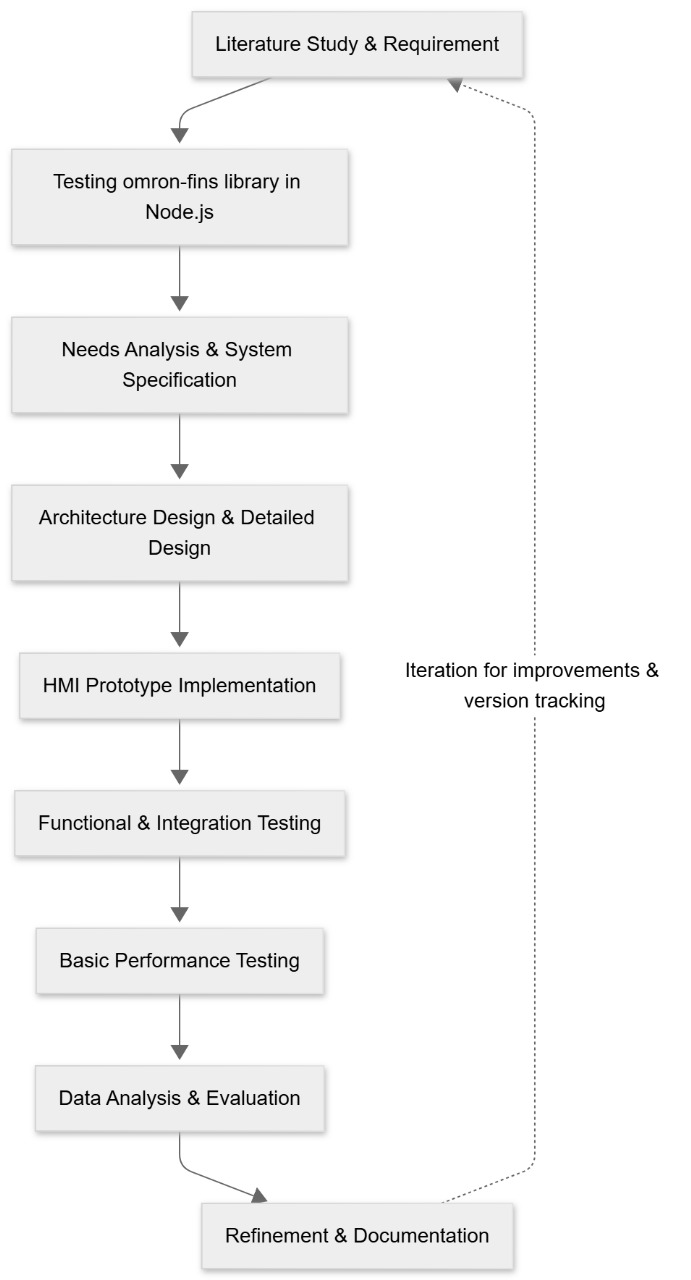
\includegraphics[width=0.24\linewidth]{images/flowchart-tahapan-en.jpeg}
\end{frame}

% =========================
% SYSTEM ARCHITECTURE
% =========================
\begin{frame}{System Architecture}
\begin{itemize}
  \item Three-layer architecture:
  \begin{itemize}
    \item Omron PLC layer
    \item Node.js backend (FUXA + DeviceFins)
    \item Angular frontend (HMI visualization)
  \end{itemize}
\end{itemize}
\end{frame}

% =========================
% ARCHITECTURE FIGURE
% =========================
\begin{frame}{Architecture Diagram}
\centering
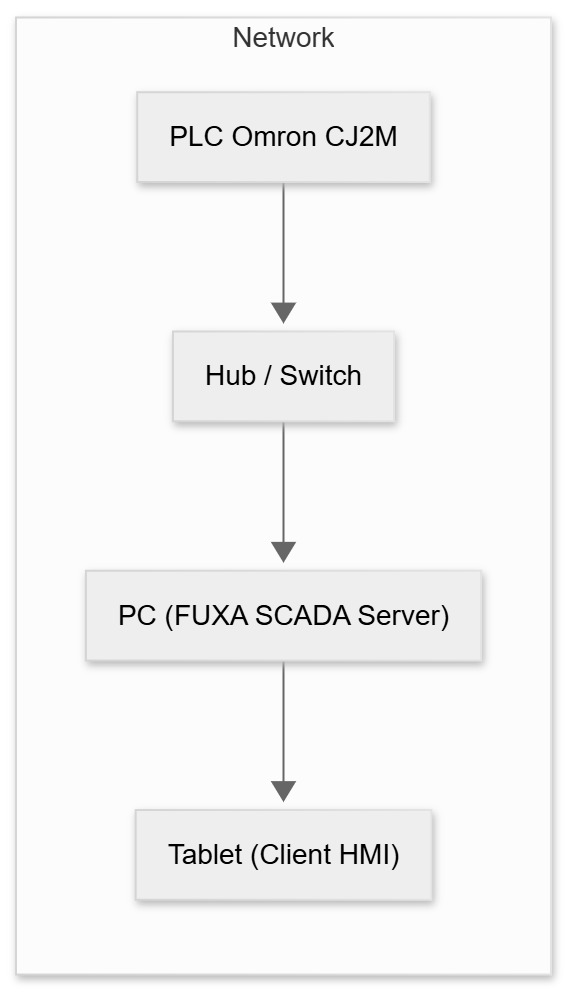
\includegraphics[width=0.8\linewidth]{images/topologi_fuxa_fins_en.jpeg}
\end{frame}

% =========================
% IMPLEMENTATION
% =========================
\begin{frame}{Implementation}
\begin{itemize}
  \item \texttt{DeviceFins} driver in Node.js backend.
  \item Supports FINS over UDP and TCP.
  \item Read/write access to DM, CIO, and W memory areas.
  \item Automatic reconnection and timeout handling.
\end{itemize}
\end{frame}

% =========================
% FRONTEND INTEGRATION
% =========================
\begin{frame}{Frontend Integration}
\begin{itemize}
  \item Device configuration (IP, port, SA1, DA1).
  \item Tag editor for FINS-specific parameters.
  \item Real-time UI updates via event emitter.
\end{itemize}
\end{frame}

% =========================
% EXPERIMENTAL SETUP
% =========================
\begin{frame}{Experimental Setup}
\begin{itemize}
  \item Omron CJ2M-CPU34 PLC.
  \item Node.js v18, FUXA v1.2.13.
  \item Stress test: 1000 reads, concurrency = 10.
  \item Metrics: latency, success rate, CPU, memory, alarms.
\end{itemize}
\end{frame}

% =========================
% KPI TABLE
% =========================
\begin{frame}{Evaluation Metrics}
\centering
\begin{tabular}{lc}
\toprule
Metric & KPI Target \\
\midrule
Latency & $\leq$200 ms \\
Success Rate & $\geq$95\% \\
CPU Usage & $\leq$30\% \\
Memory Usage & $\leq$500 MB \\
Alarm Detection & $\leq$200 ms \\
Startup Time & $\leq$10 s \\
\bottomrule
\end{tabular}
\end{frame}

% =========================
% RESULTS
% =========================
\begin{frame}{Performance Results}
\begin{itemize}
  \item Average read/write latency: \textbf{12 ms}.
  \item Communication success rate: \textbf{99\%}.
  \item CPU usage: \textbf{2\%}.
  \item Memory usage: \textbf{462 MB}.
  \item Startup time: \textbf{3.14 s}.
\end{itemize}
\end{frame}

% =========================
% ALARM ANALYSIS
% =========================
\begin{frame}{Alarm Detection Analysis}
\begin{itemize}
  \item Observed alarm detection delay: \textbf{1000 ms}.
  \item KPI target: 200 ms.
  \item Root cause: global 1-second polling interval in FUXA alarm engine.
\end{itemize}
\end{frame}

% =========================
% ALARM FIGURE
% =========================
\begin{frame}{Alarm Detection Interval}
\centering
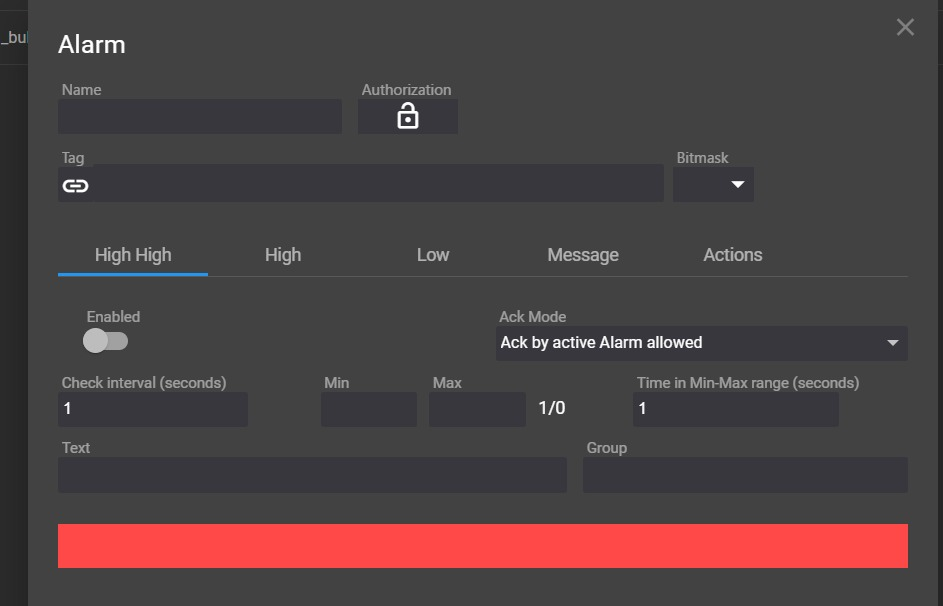
\includegraphics[width=0.8\linewidth]{images/alarm_interval.jpeg}
\end{frame}

% =========================
% COMPARISON WITH MODBUS
% =========================
\begin{frame}{Comparison with Modbus/TCP}
\begin{itemize}
  \item Comparable latency (8--15 ms).
  \item Similar reliability under LAN conditions.
  \item Alarm delay identical due to shared polling-based alarm subsystem.
\end{itemize}
\end{frame}

% =========================
% CONCLUSION
% =========================
\begin{frame}{Conclusion}
\begin{itemize}
  \item First native FINS integration for the FUXA HMI.
  \item Reliable low-latency communication with Omron PLCs.
  \item Main limitation: polling-based alarm detection delay.
\end{itemize}
\end{frame}

% =========================
% FUTURE WORK
% =========================
\begin{frame}{Future Work}
\begin{itemize}
  \item Event-driven or interrupt-based alarm handling.
  \item Enhanced security (TLS / VPN).
  \item Multi-PLC and large-scale deployment testing.
\end{itemize}
\end{frame}

% =========================
% THANK YOU
% =========================
\begin{frame}
\centering
\Huge Thank You\\[0.5cm]
\Large Questions?
\end{frame}

\end{document}
